\documentclass[10pt, a4paper,spanish]{article}
\usepackage[utf8]{inputenc}

\usepackage{varwidth}
\usepackage{graphicx}

\usepackage[T1]{fontenc} % Use 8-bit encoding that has 256 glyphs
\usepackage{microtype} % Slightly tweak font spacing for aesthetics

\usepackage[hmarginratio=1:1,top=32mm,columnsep=20pt]{geometry} % Document margins
\usepackage[hang, small,labelfont=bf,up,textfont=it,up]{caption} % Custom captions under/above floats in tables or figures
\usepackage{float} % Required for tables and figures in the multi-column environment - they need to be placed in specific locations with the [H] (e.g. \begin{table}[H])
\usepackage{hyperref} % For hyperlinks in the PDF

\usepackage{abstract} % Allows abstract customization
\renewcommand{\abstractnamefont}{\normalfont\bfseries} % Set the "Abstract" text to bold
\renewcommand{\abstracttextfont}{\normalfont\small\itshape} % Set the abstract itself to small italic text

\usepackage{titlesec} % Allows customization of titles
\renewcommand\thesection{\Roman{section}} % Roman numerals for the sections
\renewcommand\thesubsection{\Roman{subsection}} % Roman numerals for subsections
\titleformat{\section}[block]{\large\scshape\centering}{\thesection.}{1em}{} % Change the look of the section titles
\titleformat{\subsection}[block]{\large}{\thesubsection.}{1em}{} % Change the look of the section titles

\usepackage{fancyhdr} % Headers and footers
\pagestyle{fancy} % All pages have headers and footers
\fancyhead{} % Blank out the default header
\fancyfoot{} % Blank out the default footer
\fancyhead[C]{ Mayo 2016 $\bullet$ JumpVa $\bullet$ Estructura de la base de datos} % Custom header text
\fancyfoot[RO,LE]{\thepage} % Custom footer text

%----------------------------------------------------------------------------------------
%	TITLE SECTION
%----------------------------------------------------------------------------------------

\title{\vspace{-15mm}\fontsize{24pt}{10pt}\selectfont\textbf{Estructura de la base de datos}} % Article title

\author{
\large
\textsc{Alberto Amigo Alonso\textsubscript{20\%}}\\[2mm] % Your name
\textsc{Sergio Delgado Álvarez\textsubscript{20\%}}\\[2mm] % Your name
\textsc{Sergio García Prado\textsubscript{20\%}}\\[2mm] % Your name
\textsc{Oscar Fernández Angulo\textsubscript{20\%}}\\[2mm] % Your name
\textsc{Silvia Rodriguez Ares\textsubscript{20\%}}\\[2mm] % Your name
\normalsize Universidad de Valladolid \\ % Your institution
\vspace{-5mm}
}
\date{}

%----------------------------------------------------------------------------------------

\begin{document}

	\maketitle % Insert title

	\thispagestyle{fancy} % All pages have headers and footers

%----------------------------------------------------------------------------------------
%	ABSTRACT
%----------------------------------------------------------------------------------------

	\begin{abstract}
		\noindent Servicio web destinado a permitir a remitentes y destinatarios ofertar envíos para que los transportistas sean capaces de encontrarlos permitiendo a todos los usuarios monitorizarlos.
	\end{abstract}

%----------------------------------------------------------------------------------------
%	TEXT
%----------------------------------------------------------------------------------------
	\section{Casos de uso implementados}
		\paragraph{}
		Implementación de la solicitud de ingreso en el sistema, con su correspondiente acceso a la base de datos y el sistema de tokens para mantener la sesión del usuario conectado. (Las credenciales se pueden ver en el script de población de la base de datos, en la tabla Usuario).

		\paragraph{}
		Creación dinámica de la lista de envios asociados a un usuario. En este caso, aparecerán para el remitente los que se han insertado por defecto en el script de población.

		\paragraph{}
		Añadir hitos a los diferentes envios. Se pueden insertar en la base de datos nuevos hitos y dinámicamente se actualizan en la tabla principal de envios.
    \section{Descripción de la estructura de la base de datos}

    		\paragraph{}
		En la figura adjunta se muestra el esquema de las tablas resultantes del modelo E/R, con todos sus atributos, subrayadas las claves primarias y marcadas con flechas las claves ajenas.

		\paragraph{}
		A continuación se exponen las justificaciones oportunas sobre las que se basa el diseño de estas tablas:
		\begin{enumerate}
			\item Las tablas TipoHito, TipoEnvio y TipoEstado sirven para almacenar todos los códigos de este tipo de operaciones. Es decir, al existir solo cuatro tipos de envíos, en TipoEnvio se guardan las definiciones de estos cuatro tipos y desde las tablas que las referencian se puede conocer estos valores por el código, sin necesidad de almacenar de nuevo el nombre del tipo.
			\item Transportista y Remitente son especializaciones de Usuario, por lo que sobre esta última se almacena la infomación común a ambas y mediante las dos primeras se puede conocer qué tipo de usuario es cada uno a partir del email.
			\item Para conseguir los envios a los que está asociado un Transportista, es necesario usar el enlace con la tabla Puja. Esto es así porque los envios de los transportistas son referencias a los envios que un Remitente ha creado, luego habría que replicar el envío varias veces si se almacenase dentro de la tabla Envio. Esto nos proporciona una mejor gestión del espacio de almacenamiento..
		\end{enumerate}

		\begin{figure}[H]
			\centering
				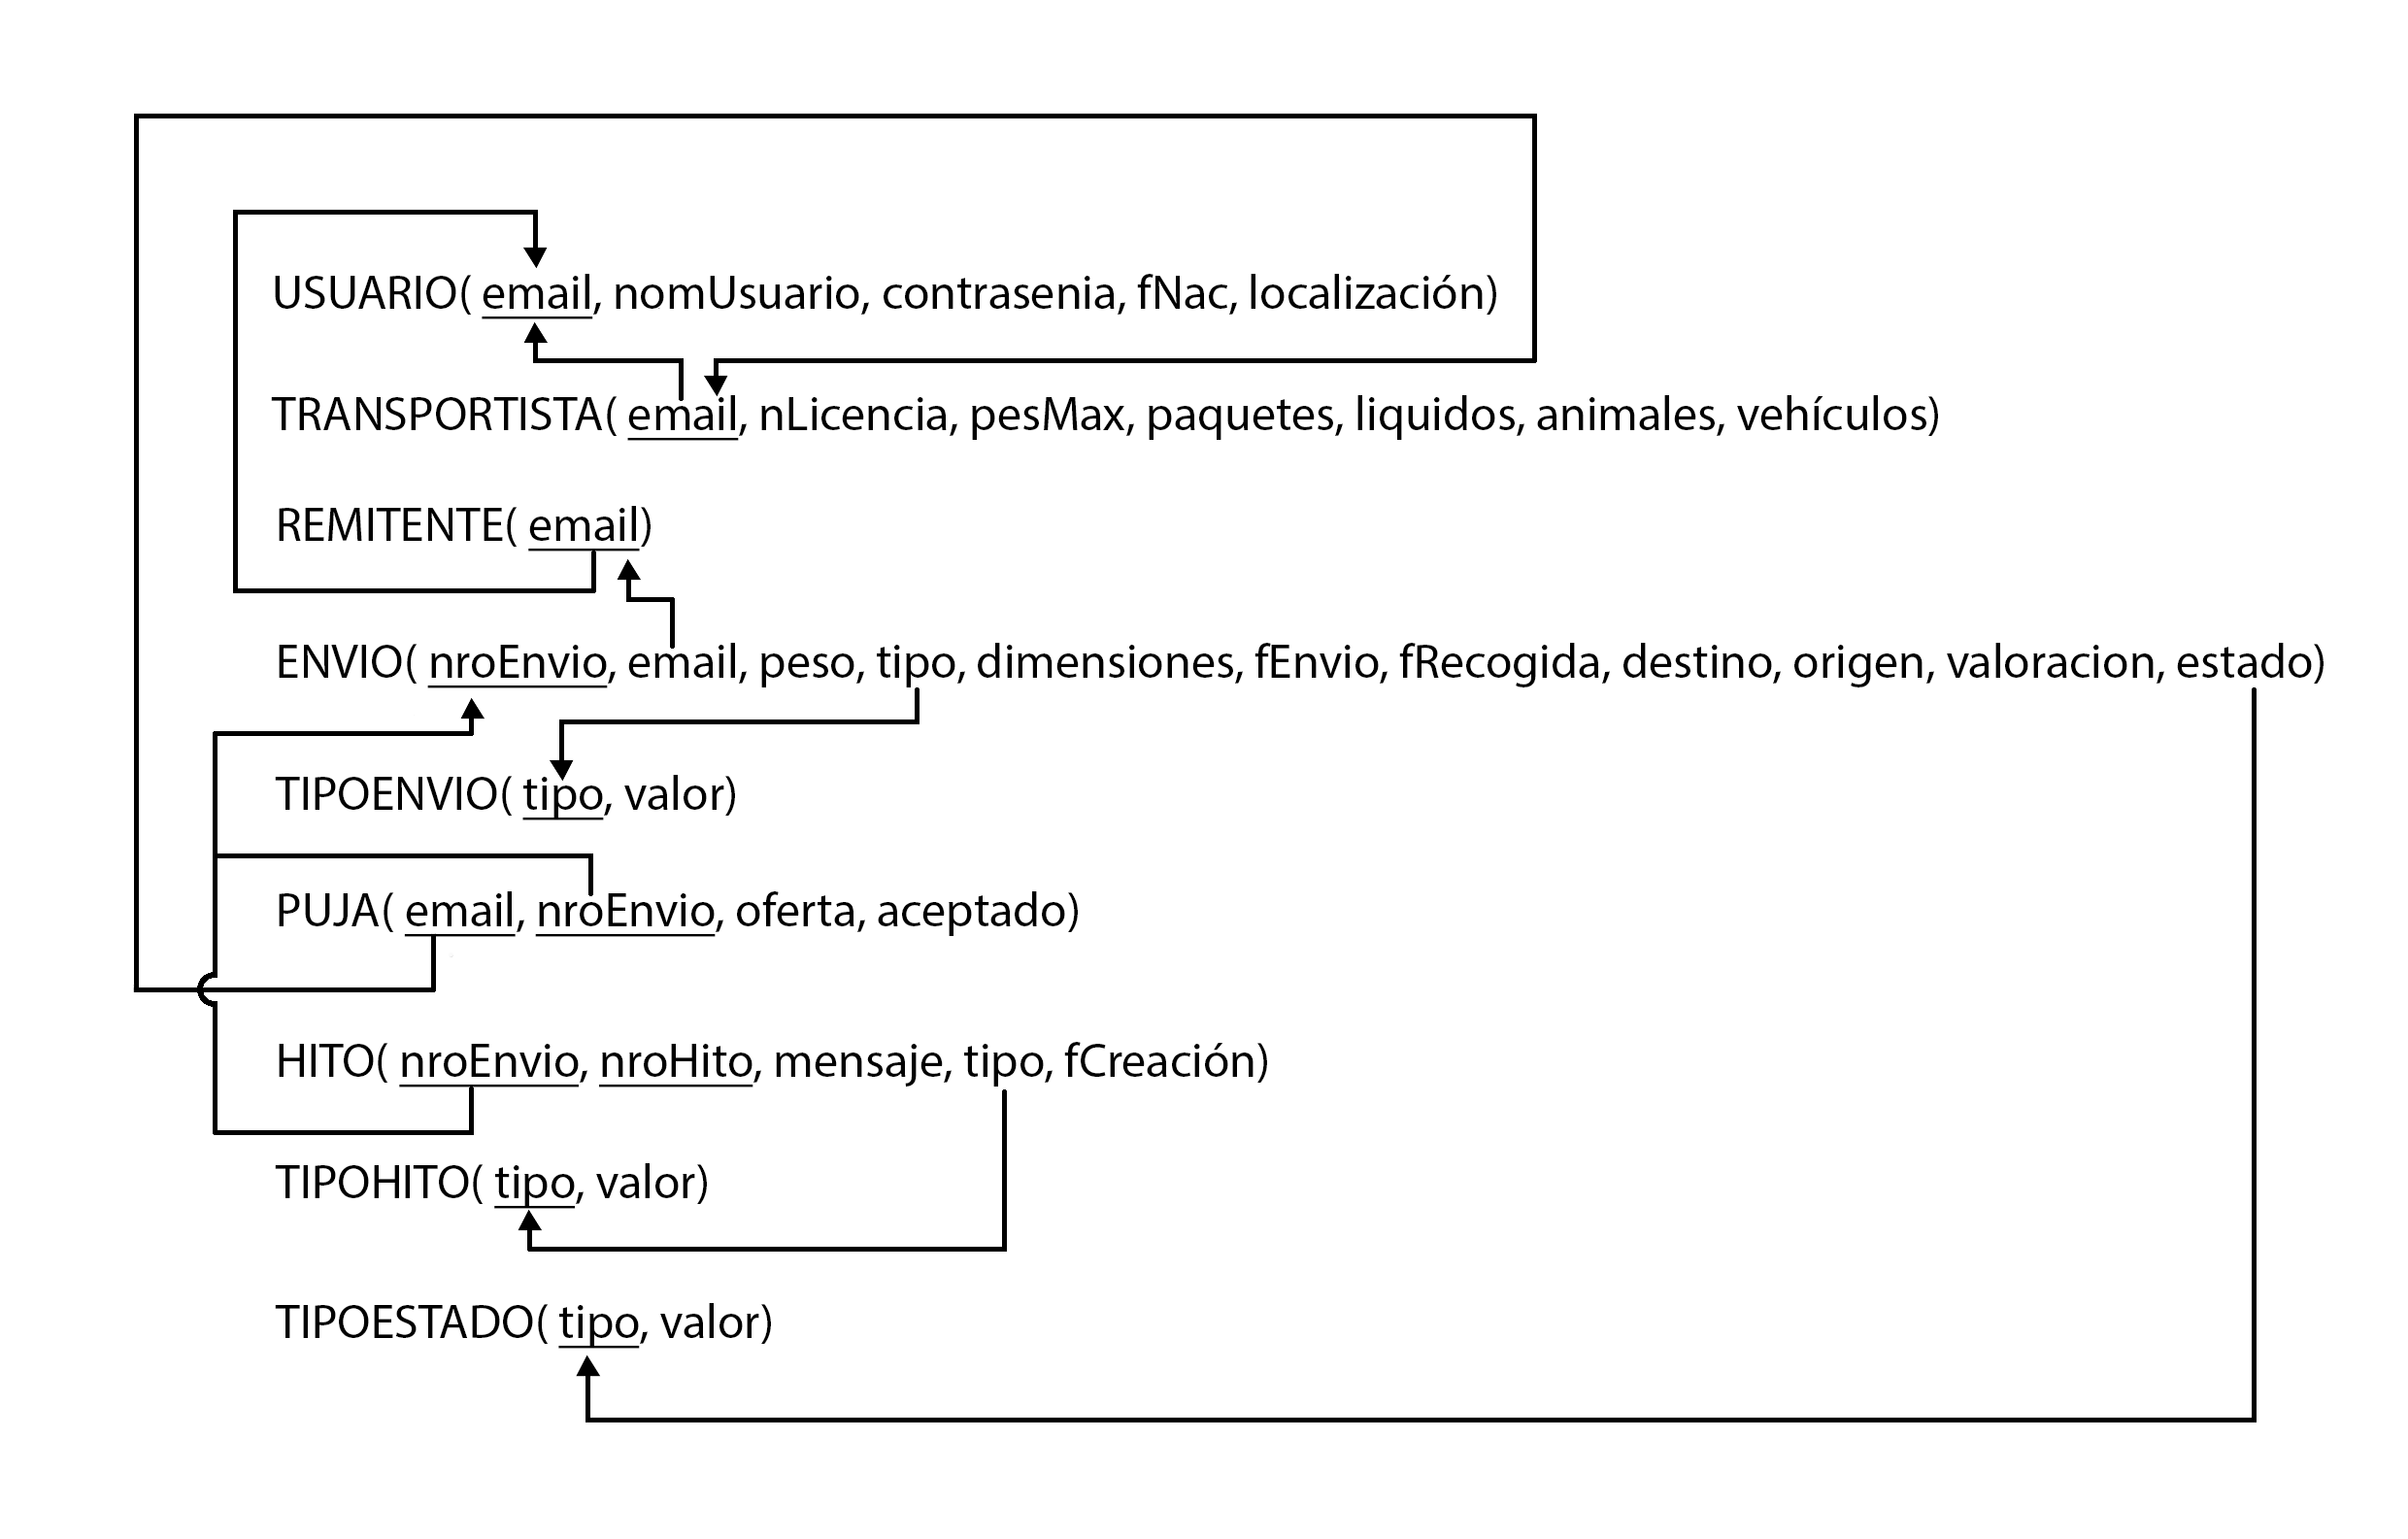
\includegraphics[width=1\textwidth]{database.png}
		\end{figure}


\end{document}
